\documentclass[10pt]{article}
%\documentclass[prd,twocolumn,showpcs,amsmath,amssymb,nofootinbib,preprintnumbers,balancelastpage,longbibliography]{revtex4-1}
\usepackage[a4paper, left=1.5cm, right=1.5cm, top=3.5cm]{geometry}
\usepackage[ngerman]{babel}
\usepackage[]{graphicx}
\usepackage{multicol}
\usepackage{amssymb}
\usepackage{inputenc}
\usepackage{breqn}
\usepackage{titlesec}
\usepackage{wrapfig}
\usepackage{blindtext}
\usepackage{lipsum}
\usepackage{caption}
\usepackage{listings}
\usepackage{fancyhdr}
\usepackage{nopageno}
\usepackage{bm}
\usepackage{authblk}
\usepackage{amsmath}
\usepackage{mathtools}
\usepackage{bm}
\usepackage[ISO]{diffcoeff}
\usepackage{xcolor}
\usepackage{csquotes}
\usepackage{siunitx}
\usepackage{circuitikz}
\usepackage{biblatex}
\usepackage{hyperref}

%%\pdfoutput=1
\usepackage{epsfig}
\usepackage{amsmath}
\usepackage{bm}
\usepackage{times}
%\usepackage{cite}
\usepackage{physics}
\usepackage{graphicx}
\usepackage{color}
\usepackage{slashed}
\usepackage{graphicx}
\usepackage{amsmath}
\usepackage{mathrsfs}
\usepackage{tikz}
\usetikzlibrary{positioning,shapes}
\usepackage{relsize,caption} 
\usepackage[latin1]{inputenc}
\usepackage{textcomp}
\usepackage[T1]{fontenc}
\usepackage{tikz}

%\usepackage{biblatex}
\usepackage{hyperref}

\usetikzlibrary{trees}
\usetikzlibrary{decorations.pathmorphing}
\usetikzlibrary{decorations.markings}
\usetikzlibrary{positioning,arrows}
\usetikzlibrary{decorations.pathmorphing}
\usetikzlibrary{decorations.markings}
\usetikzlibrary{decorations.pathreplacing,calc}
\usetikzlibrary{decorations.pathmorphing,decorations.markings,trees,positioning,arrows}   
\newif\ifmirrorsemicircle

\fancyhf[]{}

\addbibresource{latex.bib}

\newenvironment{Figure}
  {\par\medskip\noindent\minipage{\linewidth}}
  {\endminipage\par\medskip}

\begin{titlepage}
    \title{Praktikum 4 -- Versuch 443: Kernmagnetische Relaxation}
    \author[1]{Jonas Wortmann\thanks{s02jwort@uni-bonn.de}}
    \author[1]{Angelo V. Brade\thanks{s72abrad@uni-bonn.de}}
    \affil[1]{Rheinische Friedrich-Wilhelms-Universität Bonn}
    \date{\today}
\end{titlepage}

\begin{document}
\pagenumbering{gobble}
\maketitle
\newpage

\tableofcontents
\newpage

\pagenumbering{arabic}

\pagestyle{fancy}
\fancyhead[R]{\thepage}
\fancyhead[L]{\leftmark}


\begin{multicols}{2}
  \section{Einführung}
  Die Kernmagnetische Relaxation ist die Grundlage vieler moderner Messtechniken der Medizin, Chemie und Physik. Sie wird gebrauch, um z.B. MRTs oder NMRs durchzuführen. In diesem Versuch bestimmen wir die Rabioszillation und die longitudinale bzw. transversale Relaxationszeit $T_1$ und $T_2$. Diese sind materialspezifische Größen, die z.B. dessen Identifikation ermöglichen. Wir legen hier allerdings den Schwerpunkt auf die Messung der Größen selbst.
  \section{Aufbau}
  Bei dem Aufbau handelt es sich um eine Verkabelung der vier verschiedenen Geräte: MAGNET, PS2 Controller, Mainframe und das digitale Oszilloskop.
  
  Der \textbf{Magnet} ist eine Permanentmagnet, der ein homogenes Magnetfeld erzeugt. Dieser kann mit einer Helmholzspule, also zwei Spulen die genau um ihren Radius voneinander entfernt sind, ein homogenes Magnetfeld erzeugen, wenn die Spulen symmetrisch, also '$-+$' und '$-+$', oder ein Gradientenfeld, wenn die Spulen antisymmterisch, also '$-+$' und '$+-$', gepolt sind, erzeugen. Zusätzlich beinhaltet er eine sog.\ Sample Coil, die ein Magnetfeld innerhalb der Appartur messen kann. Solch ein Magnetfeld würde in unserem Fall eine Probe erzeugen, welche in die Mitte eingeführt werden kann, sodass sie umgeben von der Sample Coil und der Helmholzspulen ist. Das Innere ist nochmal in Abb. \ref{fig:mag} gezeigt.
\begin{Figure}
  \centering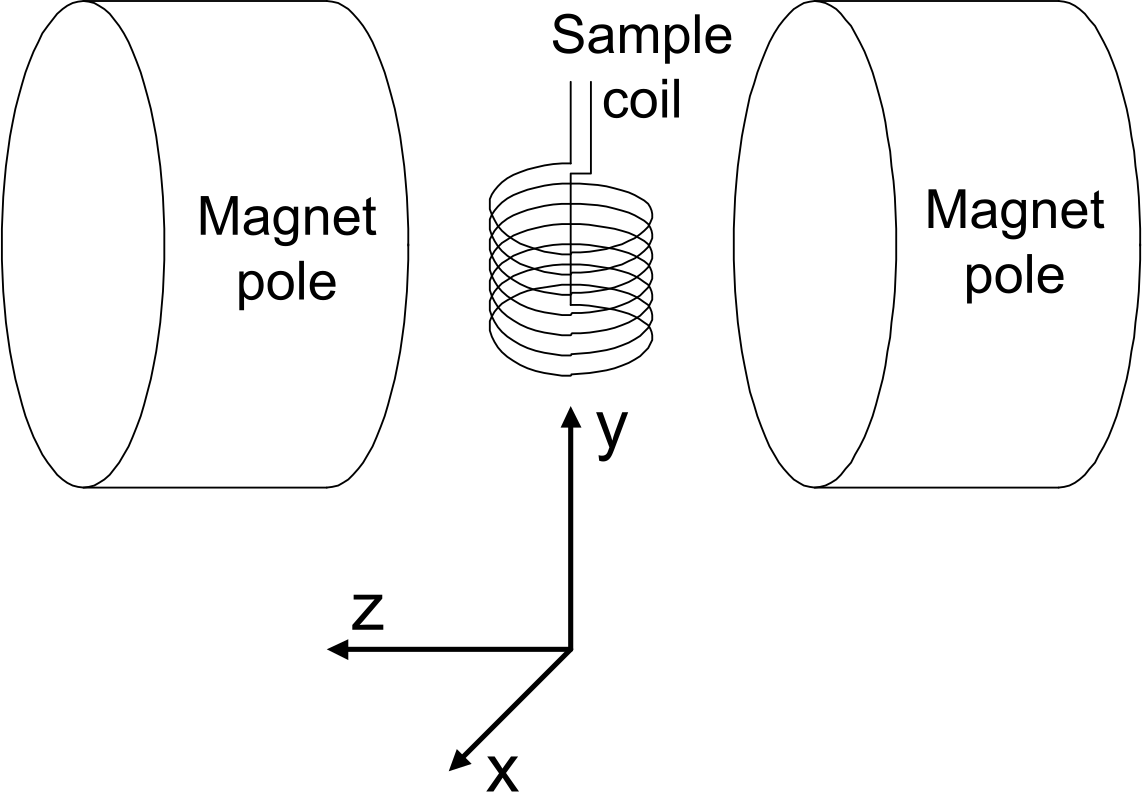
\includegraphics[width=0.8\textwidth]{magnet_aufbau.png}
  \captionof{figure}{Aufbau vom Magneten.\cite{TeachSpin}}
  \label{fig:mag}
\end{Figure}

  Der \textbf{PS2 Controller} reguliert den Magneten auf die Raumtemperatur, um Imperfektionen/Inhomogenitäten zu reduzieren. Außerdem lässt er über die Stromzufuhr der Helmholzspulen dessen Gradienten einstellen. Dafür sind uns die Regler für $X$, $Y$, $Z$ und $Z^2$ gegeben. Diese sind später bei der Justage für $\frac{\pi}{2}$- bzw. $\pi$-Pulse iterativ zu optimieren. Zusätzslich lässt sich neben der Sträke auch das Vorzeichen der Gradienten mithilfe eines jeweiligen Schalters einstellen.

  Der \textbf{Mainframe} enthält einen Receiver, der ein einkommendes Signal zur Darstellung am Oszilloskop verstärken kann, einen Synthesizer, der die Frequenz des zirkular polarisierten Mangetfeldes angibt, einen Pulse Programmer, der zwei Pulse einstellen kann und diese periodeisch wieder gibt, wobei der Abstand der zwei Pulse $\tau$ ist. Außerdem gibt es noch ein Lock-In / Field Sweep, welchen wir aber nicht benötigen.

  Das digitale \textbf{Oszilloskop} kann dann die Signal darstellen. Dafür stehen uns drei Eingänge zur verfügung. 

  \section{Durchführung}
  \subsection{Justage}
  Während des Experiments wird es einen Energiefluss vom Nukleus zum Lattice geben. Dabei erwärmt sich das Lattice. Dafür regeln wir mithilfe von zwei Potentiometern am PS2 Controller die \textbf{Temperatur}, sodass diese auf die Raumtemperatur eingestellt ist und dort konstant hällt. Ansonsten würde das Magnetfeld nicht homogen bleiben. Nun lassen sich \textbf{Tuning-Kondensatoren} an dem Magneten mithilfe eines nicht-magnetischen Schraubendrehers einstellen, um die Amplitude zu maxmieren. Hierbei wird das Signal betrachtet, wenn wir $\texttt{A_len}=\SI{2.5}{\micro s}$ und an dem Oszi einen Sweep von \SI{2}{\micro s/div} einstellen. Als Probe wird die mitgelieferte \textbf{Pickup Probe} verwendet. Das optimierte Signal ist in dem Oszillogramm von Abb. \ref{fig:PP} dargestellt.
  
\begin{Figure}
		\centering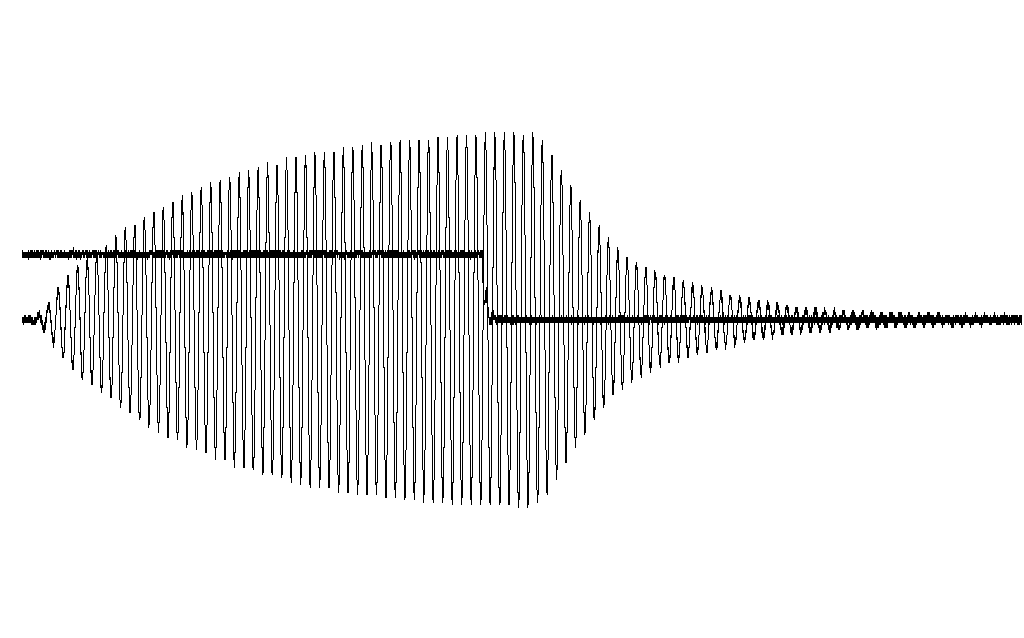
\includegraphics[width=0.8\textwidth]{scope_0.png}
    \captionof{figure}{Signal von der Pickup Probe}
		\label{fig:PP}
	\end{Figure}
Leider ist dies unser einziges gesichertes Bild von dem Singal. Eines mit korrekter Achsenbeschriftung und Skalen wurde nicht gesichert. Es ist allerdings auch hier schon gut zu erkennen, dass das größere Signal, also die Antwort der Pickup Probe, dann abfällt, sobald kein Magnetfeld (das kleine gerade Singal) anliegt.

  Um letztlich die longitunale und transversale Relaxationszeit zu ermitteln müssen wir in der Lage sein unser Medium druch die Spins mit einem Magnetfeld magnetisieren zu können. Dafür haben wir den Magneten und die Helmholzspulen. Mithilfe der Magneten können wir mit dessen homogenen Magnetfeldes eine z-Richtung defnieren und in diese auch unser Medium magnetisieren. Dabei richten sich die Spins, welche ein magnetisches Moment aufgrund des Drehimpulses der Ladung haben, in z-Richtung aus. Nun lässt sich ein zirkular polarisiertes Magenetfeld mithilfe der Helmholzspulen anlegen. Treffen wir mit der Frequenz des zirkluaren Magnetfeldes nun die sog. Lamor-Frequenz, so lässt sich ein Drehmoment auf die Spins ausüben, welches die Ausrichtung der Spins in die xy-Ebene neigt. Die Lamor-Frequen $\omega_0$ ist die gleiche, welche bei einem Übergang von $m_s=+\frac{1}{2}$ zu $m_s=-\frac{1}{2}$ benötigt wird:
\begin{align}
  \Delta U = \hbar \omega_0.
\end{align}
Um nun das Magnetfeld $B_0$ auf die Lamorfrquenz einstellen zu können, müssen wir die Energie berechnen, die uns dann den Übergang geben soll. Dafür nutzen wir die Relationen aus, dass $\bm{\mu}=\gamma \bm{J}$ und $\bm{J}=\hbar\bm{I}$ ist.
\begin{align}
  U &= - \bm{\mu} \cdot \bm{B}\\
    &= - \mu_zB_0\\
    &= - \gamma\hbar I_z B_0
\end{align}
Mit $m_s=\pm \frac{1}{2}$ erhalten wir als Differenz 
\begin{align}
  \Delta U = \gamma \hbar B_0.
\end{align}
Daraus ergibt sich die Bedingung
\begin{align}
  \omega_0 = \gamma B_0.
\end{align}
Je länger wir nun dieses Feld angeschalten lassen, desto größer wird der Neigungswinkel. Dieser Zeitraum wird RF-Pulse genannt und lässt sich an dem Pulse Programmer mit \texttt{A_len} einstellen. Sollten wir einen Neigungswinkel von $\frac{\pi}{2}$ erreichen, so können wir aufgrund der Sample Coil, die über den Reciever verstärkt wird eine Auslänkung auf unserem Oszilloskop sehen. Erreichen wir $\pi$, so wird der Ausschlag wieder 0 sein, da die Sample Coil nur ein Magnetfeld in der xy-Ebene messen kann und nun unsere Magnetisierung in $(-)$z-Richtung ausgerichtet ist. Da allerdings immernoch das homogene Magnetfeld wirkt, richtet sich der Spin nach der Neigung wieder in z-Richtung aus. Dieses Verhalten ist aufgraund der Gesammtmagnetisierung mit der Sample Coil messbar und wird Free Induction Decay (FID) genannt. Wir ersetzen hier die Pickup Probe mit unserer Mineralöl Probe. Nun müssen die Gradienten am PS2 Controller und die Frequenz am Syntheziser so optimiert werden, dass wir ein möglichst langes FID und für den Fall, dass wir bei $\pi$ liegen, eine möglichst kleine Amplitude haben. Gleichzeitig wird das I (In Phase) und Q (Out of Phase) Signal betrachetet, welches keine Nachschwingung haben darf, da dann die Resonazfrequenz getroffen wird. Wir erhalten das in Abb. \ref{fig:opt_sig} dargestellte Signal. Dabei ist eine Frequenz von \SI{21.18322+-0.00001}{\mega Hz} eingestellt. Das I und Q Signal würden dann entsprechend wie bei einem gedämpften harmonischen Oszillator im Kriechfall aussehen.
  \begin{Figure}
    \centering\resizebox{\textwidth}{!}{% GNUPLOT: LaTeX picture with Postscript
\begingroup
  \makeatletter
  \providecommand\color[2][]{%
    \GenericError{(gnuplot) \space\space\space\@spaces}{%
      Package color not loaded in conjunction with
      terminal option `colourtext'%
    }{See the gnuplot documentation for explanation.%
    }{Either use 'blacktext' in gnuplot or load the package
      color.sty in LaTeX.}%
    \renewcommand\color[2][]{}%
  }%
  \providecommand\includegraphics[2][]{%
    \GenericError{(gnuplot) \space\space\space\@spaces}{%
      Package graphicx or graphics not loaded%
    }{See the gnuplot documentation for explanation.%
    }{The gnuplot epslatex terminal needs graphicx.sty or graphics.sty.}%
    \renewcommand\includegraphics[2][]{}%
  }%
  \providecommand\rotatebox[2]{#2}%
  \@ifundefined{ifGPcolor}{%
    \newif\ifGPcolor
    \GPcolortrue
  }{}%
  \@ifundefined{ifGPblacktext}{%
    \newif\ifGPblacktext
    \GPblacktexttrue
  }{}%
  % define a \g@addto@macro without @ in the name:
  \let\gplgaddtomacro\g@addto@macro
  % define empty templates for all commands taking text:
  \gdef\gplbacktext{}%
  \gdef\gplfronttext{}%
  \makeatother
  \ifGPblacktext
    % no textcolor at all
    \def\colorrgb#1{}%
    \def\colorgray#1{}%
  \else
    % gray or color?
    \ifGPcolor
      \def\colorrgb#1{\color[rgb]{#1}}%
      \def\colorgray#1{\color[gray]{#1}}%
      \expandafter\def\csname LTw\endcsname{\color{white}}%
      \expandafter\def\csname LTb\endcsname{\color{black}}%
      \expandafter\def\csname LTa\endcsname{\color{black}}%
      \expandafter\def\csname LT0\endcsname{\color[rgb]{1,0,0}}%
      \expandafter\def\csname LT1\endcsname{\color[rgb]{0,1,0}}%
      \expandafter\def\csname LT2\endcsname{\color[rgb]{0,0,1}}%
      \expandafter\def\csname LT3\endcsname{\color[rgb]{1,0,1}}%
      \expandafter\def\csname LT4\endcsname{\color[rgb]{0,1,1}}%
      \expandafter\def\csname LT5\endcsname{\color[rgb]{1,1,0}}%
      \expandafter\def\csname LT6\endcsname{\color[rgb]{0,0,0}}%
      \expandafter\def\csname LT7\endcsname{\color[rgb]{1,0.3,0}}%
      \expandafter\def\csname LT8\endcsname{\color[rgb]{0.5,0.5,0.5}}%
    \else
      % gray
      \def\colorrgb#1{\color{black}}%
      \def\colorgray#1{\color[gray]{#1}}%
      \expandafter\def\csname LTw\endcsname{\color{white}}%
      \expandafter\def\csname LTb\endcsname{\color{black}}%
      \expandafter\def\csname LTa\endcsname{\color{black}}%
      \expandafter\def\csname LT0\endcsname{\color{black}}%
      \expandafter\def\csname LT1\endcsname{\color{black}}%
      \expandafter\def\csname LT2\endcsname{\color{black}}%
      \expandafter\def\csname LT3\endcsname{\color{black}}%
      \expandafter\def\csname LT4\endcsname{\color{black}}%
      \expandafter\def\csname LT5\endcsname{\color{black}}%
      \expandafter\def\csname LT6\endcsname{\color{black}}%
      \expandafter\def\csname LT7\endcsname{\color{black}}%
      \expandafter\def\csname LT8\endcsname{\color{black}}%
    \fi
  \fi
    \setlength{\unitlength}{0.0500bp}%
    \ifx\gptboxheight\undefined%
      \newlength{\gptboxheight}%
      \newlength{\gptboxwidth}%
      \newsavebox{\gptboxtext}%
    \fi%
    \setlength{\fboxrule}{0.5pt}%
    \setlength{\fboxsep}{1pt}%
    \definecolor{tbcol}{rgb}{1,1,1}%
\begin{picture}(7200.00,4320.00)%
    \gplgaddtomacro\gplbacktext{%
      \csname LTb\endcsname%%
      \put(731,619){\makebox(0,0)[r]{\strut{}$-0.2$}}%
      \csname LTb\endcsname%%
      \put(731,1006){\makebox(0,0)[r]{\strut{}$0$}}%
      \csname LTb\endcsname%%
      \put(731,1394){\makebox(0,0)[r]{\strut{}$0.2$}}%
      \csname LTb\endcsname%%
      \put(731,1781){\makebox(0,0)[r]{\strut{}$0.4$}}%
      \csname LTb\endcsname%%
      \put(731,2169){\makebox(0,0)[r]{\strut{}$0.6$}}%
      \csname LTb\endcsname%%
      \put(731,2556){\makebox(0,0)[r]{\strut{}$0.8$}}%
      \csname LTb\endcsname%%
      \put(731,2944){\makebox(0,0)[r]{\strut{}$1$}}%
      \csname LTb\endcsname%%
      \put(731,3331){\makebox(0,0)[r]{\strut{}$1.2$}}%
      \csname LTb\endcsname%%
      \put(731,3718){\makebox(0,0)[r]{\strut{}$1.4$}}%
      \csname LTb\endcsname%%
      \put(731,4106){\makebox(0,0)[r]{\strut{}$1.6$}}%
      \csname LTb\endcsname%%
      \put(829,425){\makebox(0,0){\strut{}$-20$}}%
      \csname LTb\endcsname%%
      \put(1380,425){\makebox(0,0){\strut{}$-15$}}%
      \csname LTb\endcsname%%
      \put(1931,425){\makebox(0,0){\strut{}$-10$}}%
      \csname LTb\endcsname%%
      \put(2481,425){\makebox(0,0){\strut{}$-5$}}%
      \csname LTb\endcsname%%
      \put(3032,425){\makebox(0,0){\strut{}$0$}}%
      \csname LTb\endcsname%%
      \put(3582,425){\makebox(0,0){\strut{}$5$}}%
      \csname LTb\endcsname%%
      \put(4133,425){\makebox(0,0){\strut{}$10$}}%
      \csname LTb\endcsname%%
      \put(4683,425){\makebox(0,0){\strut{}$15$}}%
      \csname LTb\endcsname%%
      \put(5234,425){\makebox(0,0){\strut{}$20$}}%
      \csname LTb\endcsname%%
      \put(5785,425){\makebox(0,0){\strut{}$25$}}%
      \csname LTb\endcsname%%
      \put(6335,425){\makebox(0,0){\strut{}$30$}}%
      \csname LTb\endcsname%%
      \put(6886,425){\makebox(0,0){\strut{}$35$}}%
    }%
    \gplgaddtomacro\gplfronttext{%
      \csname LTb\endcsname%%
      \put(6123,3932){\makebox(0,0)[r]{\strut{}FID}}%
      \csname LTb\endcsname%%
      \put(170,2362){\rotatebox{-270.00}{\makebox(0,0){\strut{}Auslenkung/\SI{}{V}}}}%
      \csname LTb\endcsname%%
      \put(3858,135){\makebox(0,0){\strut{}Zeit t/\SI{}{\micro s}}}%
    }%
    \gplbacktext
    \put(0,0){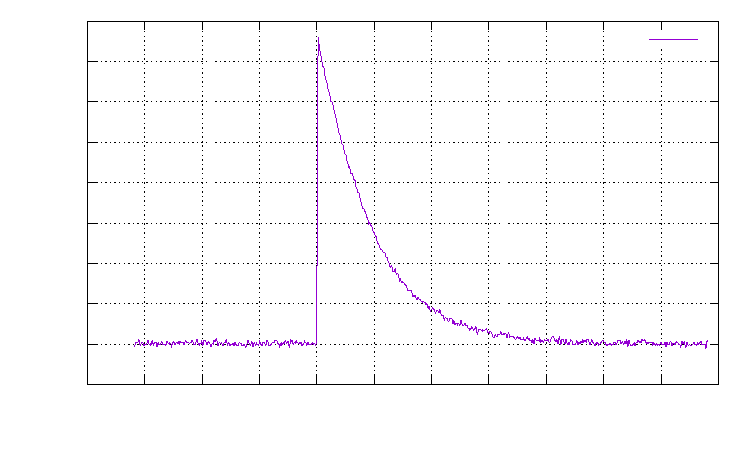
\includegraphics[width={360.00bp},height={216.00bp}]{opt_sig}}%
    \gplfronttext
  \end{picture}%
\endgroup
}
    \captionof{figure}{
      Optimiertes FID Signal.
    }
    \label{fig:opt_sig}
  \end{Figure}
  Generell messen wir aufgrund des Farady'schen Gesetzes $U=-\frac{\text{d}}{\text{d}t}\Phi_m$ eine Spannung. Das liegt daran, dass der Spin wegen des Drehimpulses um die z-Achse präzediert und so $\Phi_m$ sich zeitlich ändert. Dabei hatten wir sichergestellt, dass die Zerfallszeit über \SI{4}{\milli s} liegt.

  Nun mussten die Pulslängen ermittelt werden, dafür wurde diese so eingestellt, dass wir die Amplitude minimieren. Somit erhalten wir ein $\pi$-Puls. Währendessen verändern sich die Nachschwingungen von I und Q. Nun hablieren wir diese Pulslänge und erhalten ein $\frac{\pi}{2}$-Puls. Die Pulslängen sind dabei \SI{2.42}{\milli s} bzw. \SI{4.84}{\milli s}. Hierbei und bei allen folgenden Messungen wurde das Offset direkt im Versuch abgezogen und ist somit in der eigenen Unsicherheitenabschätzung schon mit einbezogen. Dabei erhalten wir ein Amplitudenverhältniss $U_{\text{max}}(\pi):U_{\text{max}}(\pi/2)$ von 1:\SI{17.2+-1.4} mit $U_{\text{max}}(\pi)=\SI{0.086+-0.007}{V}$ und $U_{\text{max}}(\pi/2)=\SI{1.483+-0.007}{V}$, was über den notwendigen 1:6 liegt.


  \subsection{Rabi-Oszillationen}
  Bei der Rabi-Oszillation erhöhen wir die Pulslänge und messen die Maxima, also die Amplitude. Wir stellen sicher, dass die Periode zwischen zwei Pulsen mit \SI{1}{s} ausreichend groß ist. Neben der FID Amplitude haben wir auch die Amplitude des In-Signals gemessen. Wir wählen hierbei Pulslängen von zwischen \SI{0.5}{\micro s} und \SI{12}{\micro s}. Dabei erhalten wir Abb. \ref{fig:rabioszi}.
  \begin{Figure}
    \centering\resizebox{\textwidth}{!}{% GNUPLOT: LaTeX picture with Postscript
\begingroup
  \makeatletter
  \providecommand\color[2][]{%
    \GenericError{(gnuplot) \space\space\space\@spaces}{%
      Package color not loaded in conjunction with
      terminal option `colourtext'%
    }{See the gnuplot documentation for explanation.%
    }{Either use 'blacktext' in gnuplot or load the package
      color.sty in LaTeX.}%
    \renewcommand\color[2][]{}%
  }%
  \providecommand\includegraphics[2][]{%
    \GenericError{(gnuplot) \space\space\space\@spaces}{%
      Package graphicx or graphics not loaded%
    }{See the gnuplot documentation for explanation.%
    }{The gnuplot epslatex terminal needs graphicx.sty or graphics.sty.}%
    \renewcommand\includegraphics[2][]{}%
  }%
  \providecommand\rotatebox[2]{#2}%
  \@ifundefined{ifGPcolor}{%
    \newif\ifGPcolor
    \GPcolortrue
  }{}%
  \@ifundefined{ifGPblacktext}{%
    \newif\ifGPblacktext
    \GPblacktexttrue
  }{}%
  % define a \g@addto@macro without @ in the name:
  \let\gplgaddtomacro\g@addto@macro
  % define empty templates for all commands taking text:
  \gdef\gplbacktext{}%
  \gdef\gplfronttext{}%
  \makeatother
  \ifGPblacktext
    % no textcolor at all
    \def\colorrgb#1{}%
    \def\colorgray#1{}%
  \else
    % gray or color?
    \ifGPcolor
      \def\colorrgb#1{\color[rgb]{#1}}%
      \def\colorgray#1{\color[gray]{#1}}%
      \expandafter\def\csname LTw\endcsname{\color{white}}%
      \expandafter\def\csname LTb\endcsname{\color{black}}%
      \expandafter\def\csname LTa\endcsname{\color{black}}%
      \expandafter\def\csname LT0\endcsname{\color[rgb]{1,0,0}}%
      \expandafter\def\csname LT1\endcsname{\color[rgb]{0,1,0}}%
      \expandafter\def\csname LT2\endcsname{\color[rgb]{0,0,1}}%
      \expandafter\def\csname LT3\endcsname{\color[rgb]{1,0,1}}%
      \expandafter\def\csname LT4\endcsname{\color[rgb]{0,1,1}}%
      \expandafter\def\csname LT5\endcsname{\color[rgb]{1,1,0}}%
      \expandafter\def\csname LT6\endcsname{\color[rgb]{0,0,0}}%
      \expandafter\def\csname LT7\endcsname{\color[rgb]{1,0.3,0}}%
      \expandafter\def\csname LT8\endcsname{\color[rgb]{0.5,0.5,0.5}}%
    \else
      % gray
      \def\colorrgb#1{\color{black}}%
      \def\colorgray#1{\color[gray]{#1}}%
      \expandafter\def\csname LTw\endcsname{\color{white}}%
      \expandafter\def\csname LTb\endcsname{\color{black}}%
      \expandafter\def\csname LTa\endcsname{\color{black}}%
      \expandafter\def\csname LT0\endcsname{\color{black}}%
      \expandafter\def\csname LT1\endcsname{\color{black}}%
      \expandafter\def\csname LT2\endcsname{\color{black}}%
      \expandafter\def\csname LT3\endcsname{\color{black}}%
      \expandafter\def\csname LT4\endcsname{\color{black}}%
      \expandafter\def\csname LT5\endcsname{\color{black}}%
      \expandafter\def\csname LT6\endcsname{\color{black}}%
      \expandafter\def\csname LT7\endcsname{\color{black}}%
      \expandafter\def\csname LT8\endcsname{\color{black}}%
    \fi
  \fi
    \setlength{\unitlength}{0.0500bp}%
    \ifx\gptboxheight\undefined%
      \newlength{\gptboxheight}%
      \newlength{\gptboxwidth}%
      \newsavebox{\gptboxtext}%
    \fi%
    \setlength{\fboxrule}{0.5pt}%
    \setlength{\fboxsep}{1pt}%
    \definecolor{tbcol}{rgb}{1,1,1}%
\begin{picture}(7200.00,4320.00)%
    \gplgaddtomacro\gplbacktext{%
      \csname LTb\endcsname%%
      \put(731,619){\makebox(0,0)[r]{\strut{}$-400$}}%
      \csname LTb\endcsname%%
      \put(731,967){\makebox(0,0)[r]{\strut{}$-200$}}%
      \csname LTb\endcsname%%
      \put(731,1316){\makebox(0,0)[r]{\strut{}$0$}}%
      \csname LTb\endcsname%%
      \put(731,1665){\makebox(0,0)[r]{\strut{}$200$}}%
      \csname LTb\endcsname%%
      \put(731,2014){\makebox(0,0)[r]{\strut{}$400$}}%
      \csname LTb\endcsname%%
      \put(731,2362){\makebox(0,0)[r]{\strut{}$600$}}%
      \csname LTb\endcsname%%
      \put(731,2711){\makebox(0,0)[r]{\strut{}$800$}}%
      \csname LTb\endcsname%%
      \put(731,3060){\makebox(0,0)[r]{\strut{}$1000$}}%
      \csname LTb\endcsname%%
      \put(731,3409){\makebox(0,0)[r]{\strut{}$1200$}}%
      \csname LTb\endcsname%%
      \put(731,3757){\makebox(0,0)[r]{\strut{}$1400$}}%
      \csname LTb\endcsname%%
      \put(731,4106){\makebox(0,0)[r]{\strut{}$1600$}}%
      \csname LTb\endcsname%%
      \put(829,425){\makebox(0,0){\strut{}$0$}}%
      \csname LTb\endcsname%%
      \put(1839,425){\makebox(0,0){\strut{}$2$}}%
      \csname LTb\endcsname%%
      \put(2848,425){\makebox(0,0){\strut{}$4$}}%
      \csname LTb\endcsname%%
      \put(3858,425){\makebox(0,0){\strut{}$6$}}%
      \csname LTb\endcsname%%
      \put(4867,425){\makebox(0,0){\strut{}$8$}}%
      \csname LTb\endcsname%%
      \put(5876,425){\makebox(0,0){\strut{}$10$}}%
      \csname LTb\endcsname%%
      \put(6886,425){\makebox(0,0){\strut{}$12$}}%
    }%
    \gplgaddtomacro\gplfronttext{%
      \csname LTb\endcsname%%
      \put(6123,3932){\makebox(0,0)[r]{\strut{}Probe}}%
      \csname LTb\endcsname%%
      \put(6123,3738){\makebox(0,0)[r]{\strut{}Probe fit}}%
      \csname LTb\endcsname%%
      \put(6123,3545){\makebox(0,0)[r]{\strut{}In-Phase}}%
      \csname LTb\endcsname%%
      \put(6123,3351){\makebox(0,0)[r]{\strut{}In-Phase fit}}%
      \csname LTb\endcsname%%
      \put(170,2362){\rotatebox{-270.00}{\makebox(0,0){\strut{}Amplitude/$\SI{}{\milli V}$}}}%
      \csname LTb\endcsname%%
      \put(3858,135){\makebox(0,0){\strut{}Pulslänge \texttt{A_len}/$\SI{}{\micro s}$}}%
    }%
    \gplbacktext
    \put(0,0){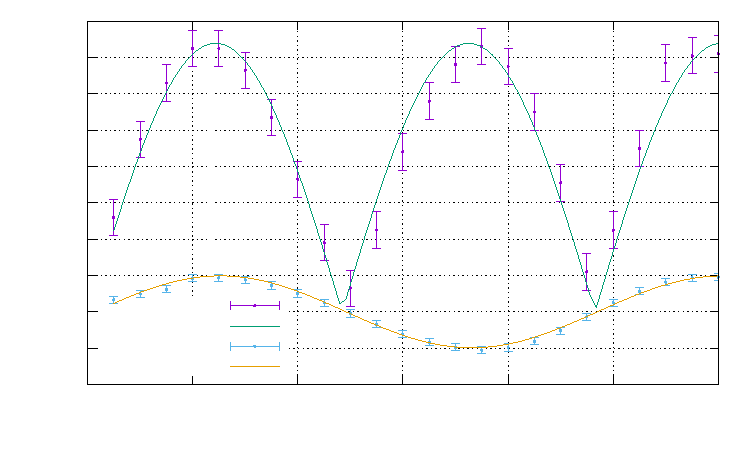
\includegraphics[width={360.00bp},height={216.00bp}]{rabi_oszi}}%
    \gplfronttext
  \end{picture}%
\endgroup
}
    \captionof{figure}{
      Rabi-Oszillation 
    }
    \label{fig:rabioszi}
  \end{Figure}
  Als Anpassfunktionen haben wir für die Probe $f(x)=m\cdot|\sin{(b\cdot x+c)}|$ und für das In-Phase Signal $g(x)=m\cdot\sin{(b\cdot x+c)}$ gewählt. Die Paramter der Anpassung sind in Tab. \ref{Tab:rabioszi} dargestellt.
  \begin{center}
    \begin{tabular}{c|cc}
    & Probe & In-Phase \\
    \hline
    red. $\chi^2$ & 1.03 & 0.46 \\
    $m$ & \SI{1478 \pm 29}{\milli\volt} & \SI{197.9 \pm 3.9}{\milli\volt} \\
    $b$ & \SI{0.6530 \pm 0.0060}{\per\micro\second} & \SI{0.6571 \pm 0.0059}{\per\micro\second} \\
    $c$ & \SI{-0.021 \pm 0.042}{} & \SI{-0.090 \pm 0.041}{}
\end{tabular}
  \captionof{table}{Parameter der Anpassung zu Rabi Oszillation}
  \label{Tab:rabioszi}
  \end{center}
  Ein gutes reduziertes $\chi^2$ liegt in der Nähe von 1. Dies ist für die Probe der Fall mit $1.03$. Für das In-Phase Signal erhalten wir $\chi^2/\text{ddof}=0.46$, was unter unseren gewollten 1 liegt, aber immernoch vertretbar ist. Somit haben wir entweder bei dem In-Phase Signal unsere Messunsicherheit unterschätzt, oder gute Messergebnisse erhalten.

  Wie erwartet, erhalten wir einen Sinus -- mit und ohne Betrag -- welcher Phasengleich ist und die gleiche Periodendauer hat. Dies liegt daran, dass das Antwortsignal den Betrag der Projektion der Magnetisierung in die xy-Ebene und das I Signal die Magnetisierung in y-Richtung zeigt.

\subsection{Longitudinale Relaxationszeit $T_1$}
Die longitudinale Relaxationszeit $T_1$ beschreibt die Spin--Lattice--Relaxationszeit.
Nachdem die Spins der Protonen in der Probe durch magnetische Wechselfelder ausgelenkt wurden, relaxieren sie nach einer Zeit $T_1$ wieder in den energetisch günstigsten Zustand; entlang der Feldlinien des homogenen Magnetfeldes.
Diese Zeit $T_1$ wird longitudinale Relaxationszeit genannt.

Um diese Zeit zu messen können die Sättigungszurückgewinnungs- (SZG) oder Polarisationszurückgewinnungsmethoden (PZG) verwendet werden. 
Beide Methoden beruhen auf der Messung eines FID nach der Spinauslenkung.

\subsubsection{Sättigungszurückgewinnung}
Die Sequenz der SZG ist
\begin{align} 
        \tfrac{\pi }{2}\rightarrow \text{FID}\rightarrow \tau \rightarrow \tfrac{\pi }{2}\rightarrow \text{FID}
.\end{align} 
Gemessen wird immer die Amplitude des FID.
Zuerst werden die Spins mit einem $\pi /2$--Puls ausgelenkt. 
Man misst einen typischen FID in dem zu erkennen ist, dass die Polarisation in der $xy$--Ebene abnimmt.

Nach einer gewissen Zeit $\tau $ werden die Spins durch einen weiteren $\pi /2$--Puls ausgelenkt. 
Ist diese Zeit $\tau =\SI{0}{s}$, so erwartet man das selbe Ergebnis wie bei einem $\pi $--Puls; die Magnetisierung in der $xy$--Ebene ist vollständig aufgehoben.
Wird allerdings eine Zeit $\tau \neq \SI{0}{s}$ gewartet, relaxieren die Spins über diesen Zeitraum $\tau $ und die Magnetisierung nimmt zuerst ab.
Der zweite $\pi /2$--Puls bewirkt dann, dass die Spins zu einem Winkel unter $\pi /2$ ausgelenkt werden, allerdings nicht ganz $\pi $, was zur Folge hat, dass sich eine Magnetisierung in der $xy$--Ebene, also auch ein FID, messen lässt.
Misst man diesen zweiten FID für verschiedene Zeiten $\tau $, lässt sich daraus auf $T_1$ schließen, da die Magnetisierung von $T_1$ abhängt.
Der Zusammenhang kann mit
\begin{align} 
        M\left(\tau \right)=M_0\left(1-\text{exp}\left(-\dfrac{\tau }{T_1}\right)\right)
\end{align} 
modelliert werden.

Wichtig im Zusammenhang mit der Messung ist, dass die Periode $P$ zwischen zwei Sequenzen groß genug ist, damit die Spins genügend Zeit haben vollständig zu relaxieren.
$P=\SI{1}{s}$ ist hier völlig ausreichend.
  \begin{Figure}
    \centering\resizebox{\textwidth}{!}{\input{s_zurück.tex}}
    \captionof{figure}{
      Zweites FID der Sättigungszurückgewinnung.
    }
    \label{fig:szurück}
  \end{Figure}
Die Daten und Fitfunktion sind in Abb.\ \ref{fig:szurück} dargestellt.
Die Fitfunktion ist charakterisiert durch folgende Parameter:
  \begin{center}
    \begin{tabular}{c|c}
    & Fit SZG\\
    \hline
    red.\ $\chi^2$ & 1.17785\\
    $M_0$ & $\SI{1496.68+-13.43}{mV}$ \\
    $T_1$ & $\SI{29.0361+-1.201}{ms}$ 
    \end{tabular}
  \captionof{table}{Parameter der Anpassung zum SZG}
  \label{Tab:SZG_para}
  \end{center}
Das optimale reduzierte $\chi ^2$ liegt bei 1; der Fit passt also sehr gut zu den gemessenen Datenpunkten.
Aus den Parametern ergibt sich dann die longitudinale Relaxationszeit zu
\begin{align} 
        T_1=\SI{29.0361+-1.201}{ms}
.\end{align} 
Dieser Wert wird im Anschluss der PZG diskutiert.

\subsubsection{Polarisationszurückgewinnung}
Die Sequenz der PZG ist
\begin{align} 
        \pi \rightarrow \tau \rightarrow \dfrac{\pi }{2}\rightarrow \text{FID}
.\end{align} 
Gemessen wird immer die Amplitude des FID.
Zuerst werden die Spins von einem $\pi $--Puls rotiert, so dass keine Magnetisierung in der $xy$--Ebene zu sehen ist.
Nach einer Zeit $\tau $ werden die Spins mit einem $\pi /2$--Puls weiter rotiert.
Für $\tau =\SI{0}{s}$ lässt sich ein typischer FID beobachten.
Wartet man eine Zeit von ungefähr $\tau \leq \SI{30}{ms}$, so erkennt man, dass die Magnetisierung in der $xy$--Ebene nicht mehr so stark ist, wie für $\tau =\SI{0}{s}$.
Das liegt daran, dass die Spins bereits über die Zeit $\tau $ rotiert haben (in Richtung der Gleichgewichtslage).
Wählt man $\tau $ so groß, dass die Spins genug Zeit hatten zu einer Stellung von $\pi /2$ zu rotieren, dann bewirkt der $\pi /2$--Puls, dass keine Magnetisierung zu messen ist.
Die Spins sind wieder um insgesamt $\pi $ rotiert.
Wählt man $\tau $ noch größer lässt sich wieder eine Magnetisierung nach dem $\pi /2$--Puls erkennen.
Für $\tau $ viel größer als bisher wird die Sequenz zu einem einfachen $\pi /2$--Puls.

Die Kurve der gemessenen Daten sieht dann analog zu der Kurve aus dem Verfahren der SZG aus, allerdings lässt sich noch die starke Abnahme der Magnetisierung für kleine $\tau \leq \SI{30}{ms}$ erkennen.
Passt man die Funktion
\begin{align} 
        M\left(\tau \right)=\left(1-2\cdot \text{ecp}\left(-\dfrac{\tau }{T_1}\right)\right)
\end{align} 
an die Daten für $\tau >\SI{30}{ms}$ an (da hier nur die Zunahme der Magnetisierung für $T_1$ wichtig ist), lässt sich $T_1$ berechnen.
Daten und Fitfunktion sind in Abb.\ \ref{fig:pzurück} dargestellt.
  \begin{Figure}
    \centering\resizebox{\textwidth}{!}{\input{p_zurück.tex}}
    \captionof{figure}{
      Zweites FID der Polarisationszurückgewinnung.
    }
    \label{fig:pzurück}
  \end{Figure}
Die Fitfunktion ist charakterisiert durch folgende Parameter
  \begin{center}
    \begin{tabular}{c|c}
    & Fit PZG\\
    \hline
    red.\ $\chi^2$ & 0.169581\\
    $M_0$ & $\SI{1521.43+-6.343}{mV}$ \\
    $T_1$ & $\SI{47.8268+-0.4078}{ms}$ 
    \end{tabular}
  \captionof{table}{Parameter der Anpassung zum PZG}
  \label{Tab:PZG_para}
  \end{center}
Das optimale reduzierte $\chi ^2$ liegt bei 1; der Fit ist also überangepasst.
Das könnte daran liegen, dass hier die Fehler zu groß geschätzt sind und die Fitfunktion dadurch in fast allen Fehlergrenzen liegt.
Aus den Parametern ergibt sich dann die longitudinale Relaxationszeit zu
\begin{align} 
        T_1=\SI{47.8268+-0.4078}{ms}
.\end{align} 

Dieser Wert weicht um circa $65\%$ von $T_1$ aus der SZG ab, ist aber für longitudinale Relaxationszeiten realistischer, da diese auch in der Größenordnung von Sekunden liegen können.
Die gemessenen Zeiten können allerdings nicht mit Literaturwerten verglichen werden, da das Mineralöl nicht bekannt ist und keine weiteren Literaturwerte angegeben sind.

Dieser große Unterschied war aber nicht zu erwarten, da die Methoden zwar unterschiedlich in der Durchführung sind, allerdings auf die Bestimmung der selben physikalischen Größe aus sind.
Der Grund dieser Diskrepanz könnte in der Überanpassung des Fits der PZG sein.
Es ist aber auch nicht auszuschließen, dass keine Fehler in der Messung unterlaufen sind.

\subsection{Transversale Relaxationszeit $T_2$}
Die transversale Relaxationszeit $T_2$ beschreibt die Spin--Spin--Relaxationszeit.
Wenn die Spins durch eine Puls ausgelenkt werden, dann lässt sich eine Gesamtmagnetisierung in der $xy$--Ebene messen.
Nach der Zeit $T_2$ ist diese Magnetisierung verschwunden.
Grund dafür ist, dass die Spins (die orthogonal zu den homogenen Magnetfeldlinien stehen) unterschiedliche \textsc{Lamor}--Präzessionsgeschwindigkeiten haben und so phasenverschoben werden.
Diese unterschiedlichen Geschwindigkeiten kommen durch kleine Inhomogenitäten im Magnetfeld zustande.
Durch diese Fluktuationen kommt es dann nach einer gewissen Zeit zu einem Ausgleich aller präzedierenden Spins, sodass keine Gesamtmagnetisierung in der $xy$--Ebene mehr zu messen ist.

Bei den transversalen Relaxationszeiten wird zwischen drei verschiedenen Zeiten unterschieden.
Die effektive $T_2^*$, die inhomogene $T_{2,\text{inhom.}}$ und der homogenen Relaxationszeit $T_2$.
Der Zusammenhang dieser drei Größen ist wie
\begin{align} 
        \dfrac{1}{T_2^*}=\dfrac{1}{T_{2,\text{inhom.}}}+\dfrac{1}{T_2}
.\end{align} 
Im folgenden wird $T_2^*$ und $T_2$ berechnet.

\subsubsection{Effektive Transversale Relaxationszeit $T_2^*$}
$T_2^*$ kann ohne großen Aufwand über einen FID gemessen werden.
Dazu wird die Fitfunktion
\begin{align} 
        M\left(t\right)=M_0\text{exp}\left(-\dfrac{t}{T_2^*}\right)
\end{align} 
verwendet.
  \begin{Figure}
    \centering\resizebox{\textwidth}{!}{% GNUPLOT: LaTeX picture with Postscript
\begingroup
  \makeatletter
  \providecommand\color[2][]{%
    \GenericError{(gnuplot) \space\space\space\@spaces}{%
      Package color not loaded in conjunction with
      terminal option `colourtext'%
    }{See the gnuplot documentation for explanation.%
    }{Either use 'blacktext' in gnuplot or load the package
      color.sty in LaTeX.}%
    \renewcommand\color[2][]{}%
  }%
  \providecommand\includegraphics[2][]{%
    \GenericError{(gnuplot) \space\space\space\@spaces}{%
      Package graphicx or graphics not loaded%
    }{See the gnuplot documentation for explanation.%
    }{The gnuplot epslatex terminal needs graphicx.sty or graphics.sty.}%
    \renewcommand\includegraphics[2][]{}%
  }%
  \providecommand\rotatebox[2]{#2}%
  \@ifundefined{ifGPcolor}{%
    \newif\ifGPcolor
    \GPcolortrue
  }{}%
  \@ifundefined{ifGPblacktext}{%
    \newif\ifGPblacktext
    \GPblacktexttrue
  }{}%
  % define a \g@addto@macro without @ in the name:
  \let\gplgaddtomacro\g@addto@macro
  % define empty templates for all commands taking text:
  \gdef\gplbacktext{}%
  \gdef\gplfronttext{}%
  \makeatother
  \ifGPblacktext
    % no textcolor at all
    \def\colorrgb#1{}%
    \def\colorgray#1{}%
  \else
    % gray or color?
    \ifGPcolor
      \def\colorrgb#1{\color[rgb]{#1}}%
      \def\colorgray#1{\color[gray]{#1}}%
      \expandafter\def\csname LTw\endcsname{\color{white}}%
      \expandafter\def\csname LTb\endcsname{\color{black}}%
      \expandafter\def\csname LTa\endcsname{\color{black}}%
      \expandafter\def\csname LT0\endcsname{\color[rgb]{1,0,0}}%
      \expandafter\def\csname LT1\endcsname{\color[rgb]{0,1,0}}%
      \expandafter\def\csname LT2\endcsname{\color[rgb]{0,0,1}}%
      \expandafter\def\csname LT3\endcsname{\color[rgb]{1,0,1}}%
      \expandafter\def\csname LT4\endcsname{\color[rgb]{0,1,1}}%
      \expandafter\def\csname LT5\endcsname{\color[rgb]{1,1,0}}%
      \expandafter\def\csname LT6\endcsname{\color[rgb]{0,0,0}}%
      \expandafter\def\csname LT7\endcsname{\color[rgb]{1,0.3,0}}%
      \expandafter\def\csname LT8\endcsname{\color[rgb]{0.5,0.5,0.5}}%
    \else
      % gray
      \def\colorrgb#1{\color{black}}%
      \def\colorgray#1{\color[gray]{#1}}%
      \expandafter\def\csname LTw\endcsname{\color{white}}%
      \expandafter\def\csname LTb\endcsname{\color{black}}%
      \expandafter\def\csname LTa\endcsname{\color{black}}%
      \expandafter\def\csname LT0\endcsname{\color{black}}%
      \expandafter\def\csname LT1\endcsname{\color{black}}%
      \expandafter\def\csname LT2\endcsname{\color{black}}%
      \expandafter\def\csname LT3\endcsname{\color{black}}%
      \expandafter\def\csname LT4\endcsname{\color{black}}%
      \expandafter\def\csname LT5\endcsname{\color{black}}%
      \expandafter\def\csname LT6\endcsname{\color{black}}%
      \expandafter\def\csname LT7\endcsname{\color{black}}%
      \expandafter\def\csname LT8\endcsname{\color{black}}%
    \fi
  \fi
    \setlength{\unitlength}{0.0500bp}%
    \ifx\gptboxheight\undefined%
      \newlength{\gptboxheight}%
      \newlength{\gptboxwidth}%
      \newsavebox{\gptboxtext}%
    \fi%
    \setlength{\fboxrule}{0.5pt}%
    \setlength{\fboxsep}{1pt}%
    \definecolor{tbcol}{rgb}{1,1,1}%
\begin{picture}(7200.00,4320.00)%
    \gplgaddtomacro\gplbacktext{%
      \csname LTb\endcsname%%
      \put(634,785){\makebox(0,0)[r]{\strut{}$0$}}%
      \csname LTb\endcsname%%
      \put(634,1615){\makebox(0,0)[r]{\strut{}$0.5$}}%
      \csname LTb\endcsname%%
      \put(634,2445){\makebox(0,0)[r]{\strut{}$1$}}%
      \csname LTb\endcsname%%
      \put(634,3276){\makebox(0,0)[r]{\strut{}$1.5$}}%
      \csname LTb\endcsname%%
      \put(634,4106){\makebox(0,0)[r]{\strut{}$2$}}%
      \csname LTb\endcsname%%
      \put(731,425){\makebox(0,0){\strut{}$-20$}}%
      \csname LTb\endcsname%%
      \put(1291,425){\makebox(0,0){\strut{}$-15$}}%
      \csname LTb\endcsname%%
      \put(1850,425){\makebox(0,0){\strut{}$-10$}}%
      \csname LTb\endcsname%%
      \put(2410,425){\makebox(0,0){\strut{}$-5$}}%
      \csname LTb\endcsname%%
      \put(2969,425){\makebox(0,0){\strut{}$0$}}%
      \csname LTb\endcsname%%
      \put(3529,425){\makebox(0,0){\strut{}$5$}}%
      \csname LTb\endcsname%%
      \put(4088,425){\makebox(0,0){\strut{}$10$}}%
      \csname LTb\endcsname%%
      \put(4648,425){\makebox(0,0){\strut{}$15$}}%
      \csname LTb\endcsname%%
      \put(5207,425){\makebox(0,0){\strut{}$20$}}%
      \csname LTb\endcsname%%
      \put(5767,425){\makebox(0,0){\strut{}$25$}}%
      \csname LTb\endcsname%%
      \put(6326,425){\makebox(0,0){\strut{}$30$}}%
      \csname LTb\endcsname%%
      \put(6886,425){\makebox(0,0){\strut{}$35$}}%
    }%
    \gplgaddtomacro\gplfronttext{%
      \csname LTb\endcsname%%
      \put(6123,3835){\makebox(0,0)[r]{\strut{}FID}}%
      \csname LTb\endcsname%%
      \put(6123,3642){\makebox(0,0)[r]{\strut{}$T_2^*$ Fit}}%
      \csname LTb\endcsname%%
      \put(170,2362){\rotatebox{-270.00}{\makebox(0,0){\strut{}Amplitude/V}}}%
      \csname LTb\endcsname%%
      \put(3809,135){\makebox(0,0){\strut{}Zeit/ms}}%
    }%
    \gplbacktext
    \put(0,0){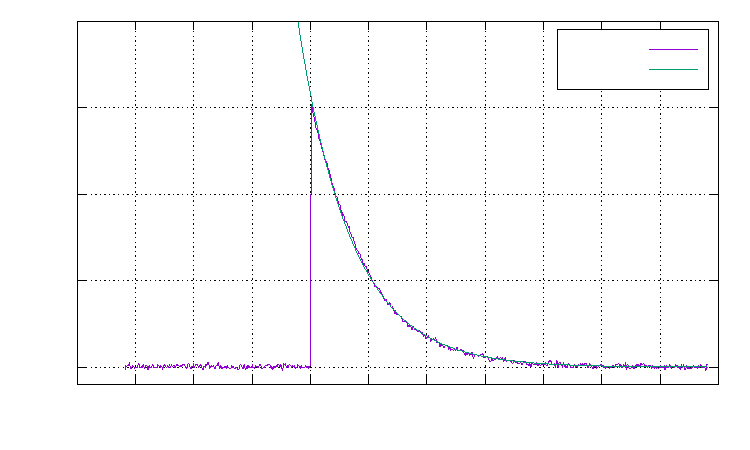
\includegraphics[width={360.00bp},height={216.00bp}]{../latex/T2eff}}%
    \gplfronttext
  \end{picture}%
\endgroup
}
    \captionof{figure}{
      FID von $T_2^*$.
    }
    \label{fig:T2eff}
  \end{Figure}
Die Fitfunktion ist charakterisiert durch folgende Parameter
  \begin{center}
    \begin{tabular}{c|c}
    & Fit $T_2^*$\\
    \hline
    $M_0$ & $\SI{1.58012+-0.002594}{V}$ \\
    $T_2^*$ & $\SI{4.63375+-0.01054}{ms}$ 
    \end{tabular}
  \captionof{table}{Parameter der Anpassung zum PZG}
  \label{Tab:PZG_para}
  \end{center}
Das reduzierte $\chi ^2$ ist hier nicht aufgeführt, da diese Datenpunkte ohne Fehler dem Oszi entnommen worden sind.
Die effektive transversale Relaxationszeit berechnet sich dann mit Hilfe des Fits zu
\begin{align} 
        T_2^*=\SI{4.63375+-0.01054}{ms}
.\end{align} 
Für diesen Wert existiert keine Literaturangabe.
Allerdings ist $T_2^*$ um eine Größenordnung kleiner als $T_1$, was erwartet war.

\subsubsection{Homogene Transversale Relaxationszeit $T_2$}
Die homogene transversale Relaxationszeit $T_2$ kann mit Hilfe drei verschiedener Verfahren berechnet werden.
Diese Verfahren werden kurz dargestellt und die berechneten Zeiten $T_2$ am Ende diskutiert.
Die Fitfunktion wird kurz mit der Hahn--Spinecho--Sequenz dargestellt, ist aber für alle Verfahren dieselbe.
\\\\\textbf{Hahn--Spinecho--Sequenz}$\quad$
Die Sequenz des Hahn--Spinecho ist
\begin{align} 
        \dfrac{\pi }{2}\rightarrow \tau \rightarrow \pi \rightarrow \text{FID}
.\end{align} 
Werden die Spins um einen $\pi /2$--Puls rotiert, so laufen ihre \textsc{Lamor}--Präzessionen aus der Phase und man kann eine abnehmende Magnetisierung in der $xy$--Ebene messen.
Werden nach kurzer Zeit $\tau $ alle Spins um $\pi $ rotiert, dann drehen sich auch ihre Phasen um, sodass sie nach der selben Zeit $\tau $ wieder zu einer Phase zusammenlaufen.
Diesen Rückgang zu einer einheitlichen Phase lässt sich dann durch eine steigende Gesamtmagnetisierung beobachten die auch als Spinecho bezeichnet wird.
Wartet man noch eine längere Zeit, so laufen die Spins wieder außer Phase und die Gesamtmagnetisierung nimmt ab.
Der gesamte Prozess dauert also $2\tau $.

Nimmt man für verschiedene Zeiten $\tau $ die Amplituden des Echos auf, so kann man mit Hilfe einer Fitfunktion,
\begin{align} 
        M\left(\tau \right)=M_0\text{exp}\left(-\dfrac{\tau }{T_2}\right)
,\end{align} 
die Zeit $T_2$ bestimmen.
  \begin{Figure}
    \centering\resizebox{\textwidth}{!}{% GNUPLOT: LaTeX picture with Postscript
\begingroup
  \makeatletter
  \providecommand\color[2][]{%
    \GenericError{(gnuplot) \space\space\space\@spaces}{%
      Package color not loaded in conjunction with
      terminal option `colourtext'%
    }{See the gnuplot documentation for explanation.%
    }{Either use 'blacktext' in gnuplot or load the package
      color.sty in LaTeX.}%
    \renewcommand\color[2][]{}%
  }%
  \providecommand\includegraphics[2][]{%
    \GenericError{(gnuplot) \space\space\space\@spaces}{%
      Package graphicx or graphics not loaded%
    }{See the gnuplot documentation for explanation.%
    }{The gnuplot epslatex terminal needs graphicx.sty or graphics.sty.}%
    \renewcommand\includegraphics[2][]{}%
  }%
  \providecommand\rotatebox[2]{#2}%
  \@ifundefined{ifGPcolor}{%
    \newif\ifGPcolor
    \GPcolortrue
  }{}%
  \@ifundefined{ifGPblacktext}{%
    \newif\ifGPblacktext
    \GPblacktexttrue
  }{}%
  % define a \g@addto@macro without @ in the name:
  \let\gplgaddtomacro\g@addto@macro
  % define empty templates for all commands taking text:
  \gdef\gplbacktext{}%
  \gdef\gplfronttext{}%
  \makeatother
  \ifGPblacktext
    % no textcolor at all
    \def\colorrgb#1{}%
    \def\colorgray#1{}%
  \else
    % gray or color?
    \ifGPcolor
      \def\colorrgb#1{\color[rgb]{#1}}%
      \def\colorgray#1{\color[gray]{#1}}%
      \expandafter\def\csname LTw\endcsname{\color{white}}%
      \expandafter\def\csname LTb\endcsname{\color{black}}%
      \expandafter\def\csname LTa\endcsname{\color{black}}%
      \expandafter\def\csname LT0\endcsname{\color[rgb]{1,0,0}}%
      \expandafter\def\csname LT1\endcsname{\color[rgb]{0,1,0}}%
      \expandafter\def\csname LT2\endcsname{\color[rgb]{0,0,1}}%
      \expandafter\def\csname LT3\endcsname{\color[rgb]{1,0,1}}%
      \expandafter\def\csname LT4\endcsname{\color[rgb]{0,1,1}}%
      \expandafter\def\csname LT5\endcsname{\color[rgb]{1,1,0}}%
      \expandafter\def\csname LT6\endcsname{\color[rgb]{0,0,0}}%
      \expandafter\def\csname LT7\endcsname{\color[rgb]{1,0.3,0}}%
      \expandafter\def\csname LT8\endcsname{\color[rgb]{0.5,0.5,0.5}}%
    \else
      % gray
      \def\colorrgb#1{\color{black}}%
      \def\colorgray#1{\color[gray]{#1}}%
      \expandafter\def\csname LTw\endcsname{\color{white}}%
      \expandafter\def\csname LTb\endcsname{\color{black}}%
      \expandafter\def\csname LTa\endcsname{\color{black}}%
      \expandafter\def\csname LT0\endcsname{\color{black}}%
      \expandafter\def\csname LT1\endcsname{\color{black}}%
      \expandafter\def\csname LT2\endcsname{\color{black}}%
      \expandafter\def\csname LT3\endcsname{\color{black}}%
      \expandafter\def\csname LT4\endcsname{\color{black}}%
      \expandafter\def\csname LT5\endcsname{\color{black}}%
      \expandafter\def\csname LT6\endcsname{\color{black}}%
      \expandafter\def\csname LT7\endcsname{\color{black}}%
      \expandafter\def\csname LT8\endcsname{\color{black}}%
    \fi
  \fi
    \setlength{\unitlength}{0.0500bp}%
    \ifx\gptboxheight\undefined%
      \newlength{\gptboxheight}%
      \newlength{\gptboxwidth}%
      \newsavebox{\gptboxtext}%
    \fi%
    \setlength{\fboxrule}{0.5pt}%
    \setlength{\fboxsep}{1pt}%
    \definecolor{tbcol}{rgb}{1,1,1}%
\begin{picture}(7200.00,4320.00)%
    \gplgaddtomacro\gplbacktext{%
      \csname LTb\endcsname%%
      \put(731,967){\makebox(0,0)[r]{\strut{}$200$}}%
      \csname LTb\endcsname%%
      \put(731,1665){\makebox(0,0)[r]{\strut{}$400$}}%
      \csname LTb\endcsname%%
      \put(731,2362){\makebox(0,0)[r]{\strut{}$600$}}%
      \csname LTb\endcsname%%
      \put(731,3060){\makebox(0,0)[r]{\strut{}$800$}}%
      \csname LTb\endcsname%%
      \put(731,3757){\makebox(0,0)[r]{\strut{}$1000$}}%
      \csname LTb\endcsname%%
      \put(829,425){\makebox(0,0){\strut{}$0$}}%
      \csname LTb\endcsname%%
      \put(1931,425){\makebox(0,0){\strut{}$10$}}%
      \csname LTb\endcsname%%
      \put(3032,425){\makebox(0,0){\strut{}$20$}}%
      \csname LTb\endcsname%%
      \put(4133,425){\makebox(0,0){\strut{}$30$}}%
      \csname LTb\endcsname%%
      \put(5234,425){\makebox(0,0){\strut{}$40$}}%
      \csname LTb\endcsname%%
      \put(6335,425){\makebox(0,0){\strut{}$50$}}%
    }%
    \gplgaddtomacro\gplfronttext{%
      \csname LTb\endcsname%%
      \put(6123,3835){\makebox(0,0)[r]{\strut{}FID Echo}}%
      \csname LTb\endcsname%%
      \put(6123,3642){\makebox(0,0)[r]{\strut{}$T_2$ Fit}}%
      \csname LTb\endcsname%%
      \put(170,2362){\rotatebox{-270.00}{\makebox(0,0){\strut{}Amplitude/mV}}}%
      \csname LTb\endcsname%%
      \put(3858,135){\makebox(0,0){\strut{}Zeit/ms}}%
    }%
    \gplbacktext
    \put(0,0){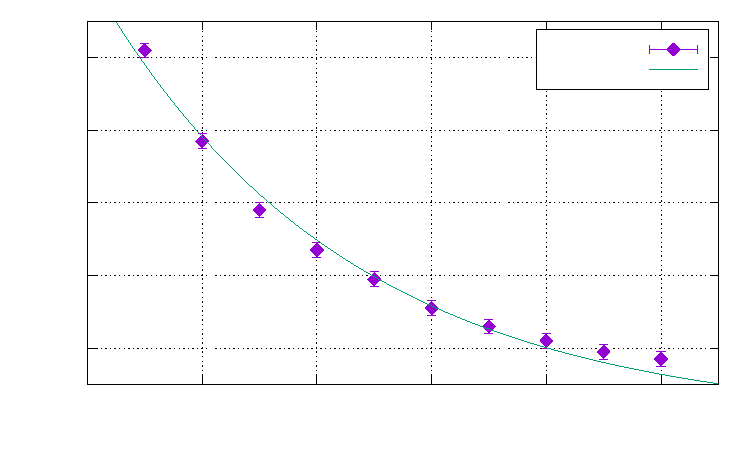
\includegraphics[width={360.00bp},height={216.00bp}]{../latex/T2hom}}%
    \gplfronttext
  \end{picture}%
\endgroup
}
    \captionof{figure}{
      Maxima der Echo FIDs von $T_2$.
    }
    \label{fig:T2eff}
  \end{Figure}
Die Fitfunktion ist charakterisiert durch folgende Parameter
  \begin{center}
    \begin{tabular}{c|c}
    & Fit $T_2$\\
    \hline
    red.\ $\chi ^2$ & 2.34122 \\
    $M_0$ & $\SI{1229.42+-39.52}{V}$ \\
    $T_2^{\text{HSE}}$ & $\SI{22.0966+-0.9622}{ms}$ 
    \end{tabular}
  \captionof{table}{Parameter der Anpassung zum Echo FID}
  \label{Tab:echo_para}
  \end{center}
Das reduzierte $\chi ^2$ liegt nahe an 1, die Abweichung kommen dadurch zustande, dass die Fehler bei dieser Messung relativ klein sind.
Die homogene transversale Relaxationszeit ist damit
\begin{align} 
        T_2^{\text{HSE}}=\SI{22.0966+-0.9622}{ms}
.\end{align} 
\\
\textbf{Carr--Purcell--Sequenz} $\quad$ 
Die Carr--Purcell--Sequenz ist
\begin{align} 
        \dfrac{\pi }{2}\rightarrow \tau \rightarrow \pi \rightarrow 2\tau \rightarrow \pi \rightarrow 2\tau \rightarrow \pi \rightarrow \hdots 
\end{align} 
Mit dieser Sequenz lassen sich mehrere Echos hintereinander beobachten.
Zuerst werden die Spins mit einem $\pi /2$--Puls in die $xy$--Ebene rotiert.
Dann wird eine Zeit $\tau $ gewartet bis ein $\pi $--Puls die Spins rotiert, um ein Echo (wie bei der Hahn--Spinecho--Sequenz) zu messen.
Wartet man $2\tau $, so werden die Ausrichtungen wieder phasenverschoben und können dann um $\pi $ rotiert werden, um ein zweites Echo zu erzeugen.
Diese Sequenz lässt sich mehrmals widerholen, um so eine Kurve wie bei der Hahn--Spinecho--Sequenz zu erhalten.

Ein Nachteil dieser Sequenz ist allerdings, dass sich die Fehler, die bei der Rotation um $\pi $ entstehen aufsummieren.
Werden die Spins nicht perfekt um $\pi $ rotiert, sondern um $\pi \pm \Delta $, so liegt die Magnetisierung nicht vollständig in der $xy$--Ebene.
Wird dann weiter um $\pi \pm \Delta $ rotiert, so läuft die Magnetisierung weiter aus der $xy$--Ebene heraus und der Fehler addiert sich.
Dieses Phänomen lässt sich in dem starken Abfall der Kurve erkennen.

Das Q--Signal ist über die ganze Sequenz gleichgerichtet, der Unterschied zur Meiboom--Gill--Sequenz wird im nächsten Abschnitt klar.
  \begin{Figure}
    \centering\resizebox{\textwidth}{!}{% GNUPLOT: LaTeX picture with Postscript
\begingroup
  \makeatletter
  \providecommand\color[2][]{%
    \GenericError{(gnuplot) \space\space\space\@spaces}{%
      Package color not loaded in conjunction with
      terminal option `colourtext'%
    }{See the gnuplot documentation for explanation.%
    }{Either use 'blacktext' in gnuplot or load the package
      color.sty in LaTeX.}%
    \renewcommand\color[2][]{}%
  }%
  \providecommand\includegraphics[2][]{%
    \GenericError{(gnuplot) \space\space\space\@spaces}{%
      Package graphicx or graphics not loaded%
    }{See the gnuplot documentation for explanation.%
    }{The gnuplot epslatex terminal needs graphicx.sty or graphics.sty.}%
    \renewcommand\includegraphics[2][]{}%
  }%
  \providecommand\rotatebox[2]{#2}%
  \@ifundefined{ifGPcolor}{%
    \newif\ifGPcolor
    \GPcolortrue
  }{}%
  \@ifundefined{ifGPblacktext}{%
    \newif\ifGPblacktext
    \GPblacktexttrue
  }{}%
  % define a \g@addto@macro without @ in the name:
  \let\gplgaddtomacro\g@addto@macro
  % define empty templates for all commands taking text:
  \gdef\gplbacktext{}%
  \gdef\gplfronttext{}%
  \makeatother
  \ifGPblacktext
    % no textcolor at all
    \def\colorrgb#1{}%
    \def\colorgray#1{}%
  \else
    % gray or color?
    \ifGPcolor
      \def\colorrgb#1{\color[rgb]{#1}}%
      \def\colorgray#1{\color[gray]{#1}}%
      \expandafter\def\csname LTw\endcsname{\color{white}}%
      \expandafter\def\csname LTb\endcsname{\color{black}}%
      \expandafter\def\csname LTa\endcsname{\color{black}}%
      \expandafter\def\csname LT0\endcsname{\color[rgb]{1,0,0}}%
      \expandafter\def\csname LT1\endcsname{\color[rgb]{0,1,0}}%
      \expandafter\def\csname LT2\endcsname{\color[rgb]{0,0,1}}%
      \expandafter\def\csname LT3\endcsname{\color[rgb]{1,0,1}}%
      \expandafter\def\csname LT4\endcsname{\color[rgb]{0,1,1}}%
      \expandafter\def\csname LT5\endcsname{\color[rgb]{1,1,0}}%
      \expandafter\def\csname LT6\endcsname{\color[rgb]{0,0,0}}%
      \expandafter\def\csname LT7\endcsname{\color[rgb]{1,0.3,0}}%
      \expandafter\def\csname LT8\endcsname{\color[rgb]{0.5,0.5,0.5}}%
    \else
      % gray
      \def\colorrgb#1{\color{black}}%
      \def\colorgray#1{\color[gray]{#1}}%
      \expandafter\def\csname LTw\endcsname{\color{white}}%
      \expandafter\def\csname LTb\endcsname{\color{black}}%
      \expandafter\def\csname LTa\endcsname{\color{black}}%
      \expandafter\def\csname LT0\endcsname{\color{black}}%
      \expandafter\def\csname LT1\endcsname{\color{black}}%
      \expandafter\def\csname LT2\endcsname{\color{black}}%
      \expandafter\def\csname LT3\endcsname{\color{black}}%
      \expandafter\def\csname LT4\endcsname{\color{black}}%
      \expandafter\def\csname LT5\endcsname{\color{black}}%
      \expandafter\def\csname LT6\endcsname{\color{black}}%
      \expandafter\def\csname LT7\endcsname{\color{black}}%
      \expandafter\def\csname LT8\endcsname{\color{black}}%
    \fi
  \fi
    \setlength{\unitlength}{0.0500bp}%
    \ifx\gptboxheight\undefined%
      \newlength{\gptboxheight}%
      \newlength{\gptboxwidth}%
      \newsavebox{\gptboxtext}%
    \fi%
    \setlength{\fboxrule}{0.5pt}%
    \setlength{\fboxsep}{1pt}%
    \definecolor{tbcol}{rgb}{1,1,1}%
\begin{picture}(7200.00,4320.00)%
    \gplgaddtomacro\gplbacktext{%
      \csname LTb\endcsname%%
      \put(731,619){\makebox(0,0)[r]{\strut{}$-0.2$}}%
      \csname LTb\endcsname%%
      \put(731,936){\makebox(0,0)[r]{\strut{}$0$}}%
      \csname LTb\endcsname%%
      \put(731,1253){\makebox(0,0)[r]{\strut{}$0.2$}}%
      \csname LTb\endcsname%%
      \put(731,1570){\makebox(0,0)[r]{\strut{}$0.4$}}%
      \csname LTb\endcsname%%
      \put(731,1887){\makebox(0,0)[r]{\strut{}$0.6$}}%
      \csname LTb\endcsname%%
      \put(731,2204){\makebox(0,0)[r]{\strut{}$0.8$}}%
      \csname LTb\endcsname%%
      \put(731,2521){\makebox(0,0)[r]{\strut{}$1$}}%
      \csname LTb\endcsname%%
      \put(731,2838){\makebox(0,0)[r]{\strut{}$1.2$}}%
      \csname LTb\endcsname%%
      \put(731,3155){\makebox(0,0)[r]{\strut{}$1.4$}}%
      \csname LTb\endcsname%%
      \put(731,3472){\makebox(0,0)[r]{\strut{}$1.6$}}%
      \csname LTb\endcsname%%
      \put(731,3789){\makebox(0,0)[r]{\strut{}$1.8$}}%
      \csname LTb\endcsname%%
      \put(731,4106){\makebox(0,0)[r]{\strut{}$2$}}%
      \csname LTb\endcsname%%
      \put(829,425){\makebox(0,0){\strut{}$-5$}}%
      \csname LTb\endcsname%%
      \put(1380,425){\makebox(0,0){\strut{}$0$}}%
      \csname LTb\endcsname%%
      \put(1931,425){\makebox(0,0){\strut{}$5$}}%
      \csname LTb\endcsname%%
      \put(2481,425){\makebox(0,0){\strut{}$10$}}%
      \csname LTb\endcsname%%
      \put(3032,425){\makebox(0,0){\strut{}$15$}}%
      \csname LTb\endcsname%%
      \put(3582,425){\makebox(0,0){\strut{}$20$}}%
      \csname LTb\endcsname%%
      \put(4133,425){\makebox(0,0){\strut{}$25$}}%
      \csname LTb\endcsname%%
      \put(4683,425){\makebox(0,0){\strut{}$30$}}%
      \csname LTb\endcsname%%
      \put(5234,425){\makebox(0,0){\strut{}$35$}}%
      \csname LTb\endcsname%%
      \put(5785,425){\makebox(0,0){\strut{}$40$}}%
      \csname LTb\endcsname%%
      \put(6335,425){\makebox(0,0){\strut{}$45$}}%
      \csname LTb\endcsname%%
      \put(6886,425){\makebox(0,0){\strut{}$50$}}%
    }%
    \gplgaddtomacro\gplfronttext{%
      \csname LTb\endcsname%%
      \put(170,2362){\rotatebox{-270}{\makebox(0,0){\strut{}Amplitude/V}}}%
      \csname LTb\endcsname%%
      \put(3858,135){\makebox(0,0){\strut{}Zeit/ms}}%
      \csname LTb\endcsname%%
      \put(6123,3835){\makebox(0,0)[r]{\strut{}CP Sequenz}}%
      \csname LTb\endcsname%%
      \put(6123,3642){\makebox(0,0)[r]{\strut{}CP Maxima}}%
      \csname LTb\endcsname%%
      \put(6123,3448){\makebox(0,0)[r]{\strut{}Q--Signal}}%
      \csname LTb\endcsname%%
      \put(6123,3255){\makebox(0,0)[r]{\strut{}CP Fit}}%
    }%
    \gplbacktext
    \put(0,0){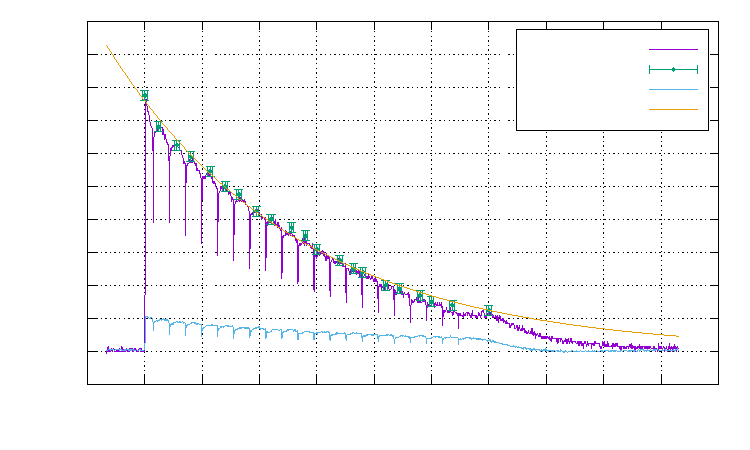
\includegraphics[width={360.00bp},height={216.00bp}]{../latex/cp}}%
    \gplfronttext
  \end{picture}%
\endgroup
}
    \captionof{figure}{
      Carr--Purcell Sequenz.
    }
    \label{fig:cp}
  \end{Figure}
  \begin{center}
    \begin{tabular}{c|c}
    & Fit $T_2$\\
    \hline
    red.\ $\chi ^2$ &  0.0183232\\
    $M_0$ & $\SI{1.51687+-0.01545}{V}$ \\
    $T_2^{\text{CP}}$ & $\SI{16.6177+-0.3026}{ms}$ 
    \end{tabular}
  \captionof{table}{Parameter der Anpassung von den Maxima der Carr--Purcell--Sequenz}
  \label{Tab:mg_para}
  \end{center}
Das reduzierte $\chi ^2$ ist viel kleiner als 1; betrachtet man allerdings die Fitfunktion lässt sich aber erkennen, dass die Fehler groß genug sind, die Funktion nur sehr genau jeden Wert trifft.
Die homogene transversale Relaxationszeit ist damit
\begin{align} 
        T_2^{\text{CP}}=\SI{16.6177+-0.3026}{ms}
\end{align} 
\\\textbf{Meiboom--Gill--Sequenz} $\quad$ 
Die Meiboom--Gill--Sequenz ist 
\begin{align} 
        \dfrac{\pi }{2}\rightarrow \tau \rightarrow +\pi \rightarrow 2\tau \rightarrow -\pi \rightarrow 2\tau \rightarrow +\pi \rightarrow \hdots 
\end{align} 
Diese Sequenz ist analog zu der Carr--Purcell--Sequenz, gleicht aber durch die alternierenden Rotationsrichtungen (dargestellt durch $\pm \pi $) die Aufsummierung des Fehlers auf.
Die Rotation ist auch hier nicht perfekt, man rotiert also um $\pi \pm \Delta $, allerdings kann dieser Fehler minimiert werden, indem man anschließend in die andere Richtung rotiert.
Die Auswirkung lassen sich an der Kurve erkennen, die eine signifikant kleinere Steigung hat; die Magnetisierung in der $xy$--Ebene nimmt also langsamer ab.

Das Q--Signal ist bei der Meiboom--Gill--Sequenz alternierend.
Man erkennt klar den Unterschied zur Carr--Purcell--Sequenz.
  \begin{Figure}
    \centering\resizebox{\textwidth}{!}{% GNUPLOT: LaTeX picture with Postscript
\begingroup
  \makeatletter
  \providecommand\color[2][]{%
    \GenericError{(gnuplot) \space\space\space\@spaces}{%
      Package color not loaded in conjunction with
      terminal option `colourtext'%
    }{See the gnuplot documentation for explanation.%
    }{Either use 'blacktext' in gnuplot or load the package
      color.sty in LaTeX.}%
    \renewcommand\color[2][]{}%
  }%
  \providecommand\includegraphics[2][]{%
    \GenericError{(gnuplot) \space\space\space\@spaces}{%
      Package graphicx or graphics not loaded%
    }{See the gnuplot documentation for explanation.%
    }{The gnuplot epslatex terminal needs graphicx.sty or graphics.sty.}%
    \renewcommand\includegraphics[2][]{}%
  }%
  \providecommand\rotatebox[2]{#2}%
  \@ifundefined{ifGPcolor}{%
    \newif\ifGPcolor
    \GPcolortrue
  }{}%
  \@ifundefined{ifGPblacktext}{%
    \newif\ifGPblacktext
    \GPblacktexttrue
  }{}%
  % define a \g@addto@macro without @ in the name:
  \let\gplgaddtomacro\g@addto@macro
  % define empty templates for all commands taking text:
  \gdef\gplbacktext{}%
  \gdef\gplfronttext{}%
  \makeatother
  \ifGPblacktext
    % no textcolor at all
    \def\colorrgb#1{}%
    \def\colorgray#1{}%
  \else
    % gray or color?
    \ifGPcolor
      \def\colorrgb#1{\color[rgb]{#1}}%
      \def\colorgray#1{\color[gray]{#1}}%
      \expandafter\def\csname LTw\endcsname{\color{white}}%
      \expandafter\def\csname LTb\endcsname{\color{black}}%
      \expandafter\def\csname LTa\endcsname{\color{black}}%
      \expandafter\def\csname LT0\endcsname{\color[rgb]{1,0,0}}%
      \expandafter\def\csname LT1\endcsname{\color[rgb]{0,1,0}}%
      \expandafter\def\csname LT2\endcsname{\color[rgb]{0,0,1}}%
      \expandafter\def\csname LT3\endcsname{\color[rgb]{1,0,1}}%
      \expandafter\def\csname LT4\endcsname{\color[rgb]{0,1,1}}%
      \expandafter\def\csname LT5\endcsname{\color[rgb]{1,1,0}}%
      \expandafter\def\csname LT6\endcsname{\color[rgb]{0,0,0}}%
      \expandafter\def\csname LT7\endcsname{\color[rgb]{1,0.3,0}}%
      \expandafter\def\csname LT8\endcsname{\color[rgb]{0.5,0.5,0.5}}%
    \else
      % gray
      \def\colorrgb#1{\color{black}}%
      \def\colorgray#1{\color[gray]{#1}}%
      \expandafter\def\csname LTw\endcsname{\color{white}}%
      \expandafter\def\csname LTb\endcsname{\color{black}}%
      \expandafter\def\csname LTa\endcsname{\color{black}}%
      \expandafter\def\csname LT0\endcsname{\color{black}}%
      \expandafter\def\csname LT1\endcsname{\color{black}}%
      \expandafter\def\csname LT2\endcsname{\color{black}}%
      \expandafter\def\csname LT3\endcsname{\color{black}}%
      \expandafter\def\csname LT4\endcsname{\color{black}}%
      \expandafter\def\csname LT5\endcsname{\color{black}}%
      \expandafter\def\csname LT6\endcsname{\color{black}}%
      \expandafter\def\csname LT7\endcsname{\color{black}}%
      \expandafter\def\csname LT8\endcsname{\color{black}}%
    \fi
  \fi
    \setlength{\unitlength}{0.0500bp}%
    \ifx\gptboxheight\undefined%
      \newlength{\gptboxheight}%
      \newlength{\gptboxwidth}%
      \newsavebox{\gptboxtext}%
    \fi%
    \setlength{\fboxrule}{0.5pt}%
    \setlength{\fboxsep}{1pt}%
    \definecolor{tbcol}{rgb}{1,1,1}%
\begin{picture}(7200.00,4320.00)%
    \gplgaddtomacro\gplbacktext{%
      \csname LTb\endcsname%%
      \put(731,619){\makebox(0,0)[r]{\strut{}$-0.2$}}%
      \csname LTb\endcsname%%
      \put(731,1006){\makebox(0,0)[r]{\strut{}$0$}}%
      \csname LTb\endcsname%%
      \put(731,1394){\makebox(0,0)[r]{\strut{}$0.2$}}%
      \csname LTb\endcsname%%
      \put(731,1781){\makebox(0,0)[r]{\strut{}$0.4$}}%
      \csname LTb\endcsname%%
      \put(731,2169){\makebox(0,0)[r]{\strut{}$0.6$}}%
      \csname LTb\endcsname%%
      \put(731,2556){\makebox(0,0)[r]{\strut{}$0.8$}}%
      \csname LTb\endcsname%%
      \put(731,2944){\makebox(0,0)[r]{\strut{}$1$}}%
      \csname LTb\endcsname%%
      \put(731,3331){\makebox(0,0)[r]{\strut{}$1.2$}}%
      \csname LTb\endcsname%%
      \put(731,3718){\makebox(0,0)[r]{\strut{}$1.4$}}%
      \csname LTb\endcsname%%
      \put(731,4106){\makebox(0,0)[r]{\strut{}$1.6$}}%
      \csname LTb\endcsname%%
      \put(829,425){\makebox(0,0){\strut{}$-5$}}%
      \csname LTb\endcsname%%
      \put(1380,425){\makebox(0,0){\strut{}$0$}}%
      \csname LTb\endcsname%%
      \put(1931,425){\makebox(0,0){\strut{}$5$}}%
      \csname LTb\endcsname%%
      \put(2481,425){\makebox(0,0){\strut{}$10$}}%
      \csname LTb\endcsname%%
      \put(3032,425){\makebox(0,0){\strut{}$15$}}%
      \csname LTb\endcsname%%
      \put(3582,425){\makebox(0,0){\strut{}$20$}}%
      \csname LTb\endcsname%%
      \put(4133,425){\makebox(0,0){\strut{}$25$}}%
      \csname LTb\endcsname%%
      \put(4683,425){\makebox(0,0){\strut{}$30$}}%
      \csname LTb\endcsname%%
      \put(5234,425){\makebox(0,0){\strut{}$35$}}%
      \csname LTb\endcsname%%
      \put(5785,425){\makebox(0,0){\strut{}$40$}}%
      \csname LTb\endcsname%%
      \put(6335,425){\makebox(0,0){\strut{}$45$}}%
      \csname LTb\endcsname%%
      \put(6886,425){\makebox(0,0){\strut{}$50$}}%
    }%
    \gplgaddtomacro\gplfronttext{%
      \csname LTb\endcsname%%
      \put(170,2362){\rotatebox{-270}{\makebox(0,0){\strut{}Amplitude/V}}}%
      \csname LTb\endcsname%%
      \put(3858,135){\makebox(0,0){\strut{}Zeit/ms}}%
      \csname LTb\endcsname%%
      \put(6123,3835){\makebox(0,0)[r]{\strut{}MG Sequenz}}%
      \csname LTb\endcsname%%
      \put(6123,3642){\makebox(0,0)[r]{\strut{}MG Maxima}}%
      \csname LTb\endcsname%%
      \put(6123,3448){\makebox(0,0)[r]{\strut{}Q--Signal}}%
      \csname LTb\endcsname%%
      \put(6123,3255){\makebox(0,0)[r]{\strut{}MG Fit}}%
    }%
    \gplbacktext
    \put(0,0){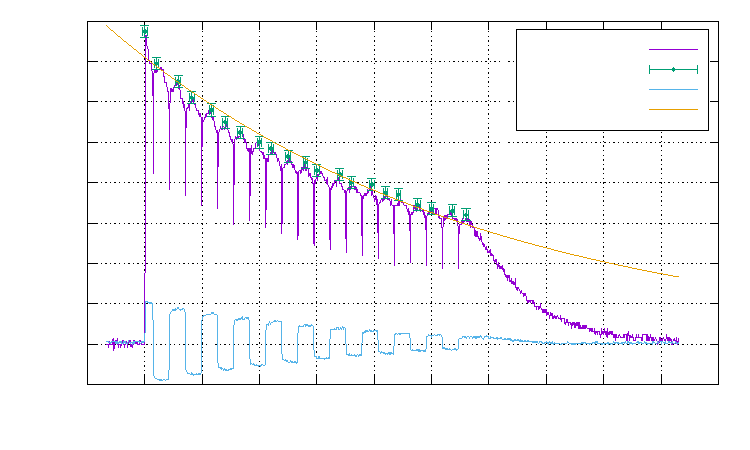
\includegraphics[width={360.00bp},height={216.00bp}]{../latex/mg}}%
    \gplfronttext
  \end{picture}%
\endgroup
}
    \captionof{figure}{
      Meiboom--Gill Sequenz.
    }
    \label{fig:mg}
  \end{Figure}
  \begin{center}
    \begin{tabular}{c|c}
    & Fit $T_2$\\
    \hline
    red.\ $\chi ^2$ &  0.0446407\\
    $M_0$ & $\SI{1.42096+-0.02117}{V}$ \\
    $T_2^{\text{MG}}$ & $\SI{32.0455+-1.228}{ms}$ 
    \end{tabular}
  \captionof{table}{Parameter der Anpassung von den Maxima der Meiboom--Gill--Sequenz}
  \label{Tab:mg_para}
  \end{center}
Das reduzierte $\chi ^2$ ist auch für diesen Fit viel zu klein; die Fehler sind allerdings passend gewählt, die Funktion trifft die Werte sehr genau.
Die homogene transversale Relaxationszeit ist damit
\begin{align} 
        T_2^{\text{MG}}=\SI{32.0455+-1.228}{ms}
.\end{align} 
\\\textbf{Vergleich} $\quad$ 
Die aus den drei Verfahren berechneten Werte sind
\begin{align} 
        T_2^{\text{HSE}}&=\SI{22.0966+-0.9622}{ms}\\
        T_2^{\text{CP}}&=\SI{16.6177+-0.3026}{ms}\\
        T_2^{\text{MG}}&=\SI{32.0455+-1.228}{ms}\\
        \overline{T_2}&=\SI{23.5866+-0.5297}{ms}
\end{align} 
Diese Werte haben sehr große Abweichungen voneinander; man erkennt $T_2^{\text{MG}}\approx 2T_2^{\text{CP}}$. Grund für diese unterschiedlichen Werte könnte folgender sein.

Da bei der Carr--Purcell--Sequenz die Fehler, die durch nicht exakte $\pi $--Pulse entstehen, aufsummiert werden, fällt die Kurve zu schnell ab.
Der Wert für $T_2$ wird dadurch verfälscht und hängt noch von der Größe der Fehler ab.
Diese Annahme basiert darauf, dass bei der Meiboom--Gill--Sequenz eine wesentlich höhere Zeit gemessen worden ist.
Diese Sequenz verwendet alternierende $\pi $--Pulse, wodurch sich der Fehler stark minimiert, was dazu führt dass die Kurve weniger stark abfällt und der Wert für $T_2$ näher am echten Wert liegt.
Vergleicht man beide Werte mit der Hahn--Spinecho--Sequenz, so erkennt man, dass sie ungefähr gleich stark von der gemessenen Zeit $T_2^{\text{HSE}}$ abweichen.
$T_2^{\text{HSE}}$ liegt also unweigerlich nah an dem Mittelwert.
$T_2^{\text{HSE}}$ wird wahrscheinlich näher am echten Wert für $T_2$ liegen, da die Zeit $\tau $ zwischen den Pulsen variiert werden kann und damit jedes Echo einzeln gemessen wird.
So erlangt man eine höhere Genauigkeit.

Dieser Wert scheint sehr nah an dem Wert von $T_1$ zu liegen, was eigentlich nicht der Fall sein sollte, da der Ausgleich durch die Phasenverschiedenheit schneller sein ist, als die Ausrichtung entlang der Feldlinien.
Da aber hier und im Folgenden kein Literaturwert gegeben und die Zusammensetzung des Mineralöls nicht bekannt ist, können die Werte nur untereinander verglichen werden.

Die Relaxationszeit, die sich aufgrund der Inhomogenitäten im Magnetfeld ergibt, kann jetzt berechnet werden mit
\begin{align} 
        \dfrac{1}{T_2^*}=\dfrac{1}{T_{2,\text{inhom}}}+\dfrac{1}{\overline{T_2}}\quad \Leftrightarrow \quad T_{2,\text{inhom}}=-\dfrac{T_2^*\overline{T_2}}{T_2^*-\overline{T_2}}
,\end{align} 
und Fehler 
\begin{align} 
        \Delta T_{2,\text{inhom}}=\,\sqrt[]{\left(\dfrac{\overline{T_2}^2}{\left(T_2^*-\overline{T_2}\right)^2}\Delta T_2^*\right)^2+\left(-\dfrac{T_2^{*2}}{\left(T_2^*-\overline{T_2}\right)^2}\Delta \overline{T_2}\right)^2}
.\end{align} 
Es ergibt sich ein Wert von
\begin{align} 
        T_{2,\text{inhom}}=\SI{5.76665+-.03562}{ms}
.\end{align} 
Man erkennt, dass die Inhomogenitäten des Magnetfeldes nicht unerheblich zur transversalen Relaxationszeit beitragen.

\section{Fazit}
In diesem Versuch wurden die Protonen in einer Mineralölprobe auf ihre longitudinalen und transversalen Relaxationszeiten untersucht.

Hierfür wurde die Probe in ein homogenes Magnetfeld eingeführt, sodass sich die Protonenspins entlang der Feldlinien ausrichten, und mit Hilfe von magnetischen Wechselfeldern konnten diese Ausgelenkt werden, um so eine Gesamtmagnetisierung in der orthogonalen Ebene zu messen.

Diese magnetischen Wechselfelder, genauer die Pulslängen der Felder, wurden mit Hilfe der \textsc{Rabi}--Oszillation eingestellt.
Trägt man die Magnetisierung in der Ebene gegen die Pulslänge auf, so konnte erfolgreich die Länge des Pulses abgelesen werden, bei der die Magnetisierung am größten ist (dies entspricht einem $\pi /2$--Puls), bzw.\ bei der die Magnetisierung verschwindet (dies entspricht einem $\pi $--Puls).

Die Gesamtmagnetisierung in der Ebene klingt nach einer gewissen Zeit ab.
Das geschieht einerseits durch die longitudinale Relaxation, bei der sich die Spins wieder entlang der homogenen Magnetfeldlinien ausrichten.
Die Dauer dieses Prozesses wurde berechnet, indem man den Free Induction Decay gemessen hat.
Der Wert liegt bei
\begin{align} 
        T_1=\SI{29.0361+-1.201}{ms}
.\end{align} 
Andererseits nimmt die Magnetisierung auch mit den unterschiedlichen \textsc{Lamor}--Präzessionsgeschwindigkeiten in der Ebene ab.
Die Zeit bis sich alle Spin aufgrund ihrer verschiedenen Phasen ausgeglichen haben wurde berechnet zu
\begin{align} 
        \overline{T_2}&=\SI{23.5866+-0.5297}{ms}
.\end{align} 


\end{multicols}
\printbibliography

\end{document}
